\documentclass[answers]{exam}
\usepackage{../HT2025}
\usepackage{graphicx}
\graphicspath{ {./images/} }

\title{Numerical Analysis -- Sheet 4\\Solving initial value problems}
\author{YOUR NAME HERE :)}
\date{Hilary Term 2025}
% version uploaded 2024-07-26


\begin{document}
\maketitle

\begin{questions}

\question%1
Consider the scalar IVP $y'=\sin(x^2) y$, $y(0)=1$. Compute the approximation of $y(0.1)$ obtained using one step of the (i) explicit Euler method, (ii) implicit Euler method, and (iii) implicit Midpoint rule. (Below is a plot of the approximate solutions along with the exact one.)
\begin{center}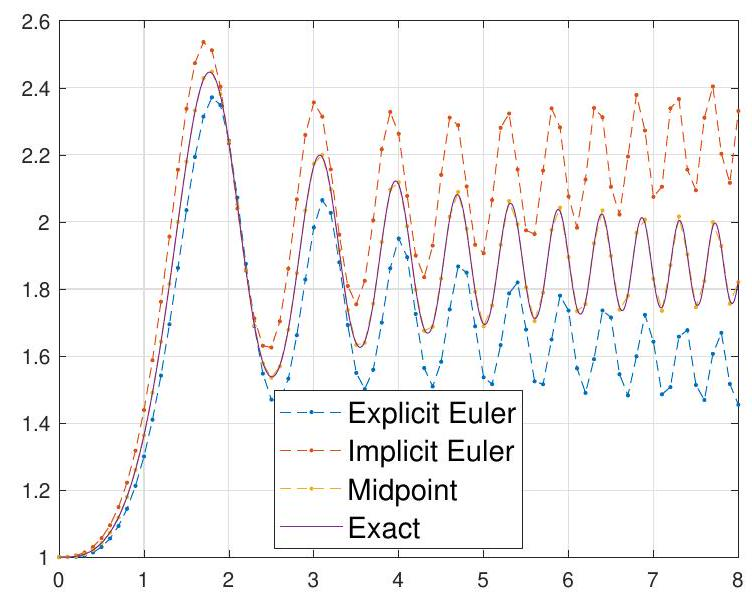
\includegraphics[width=8cm]{sheet 4 q 1}\end{center}



\question%2
Consider the autonomous ODE $\mathbf{y}'=\mathbf{f}(\mathbf{y})$ and compute the consistency order of the explicit Euler method.



\question%3
Write the formula of the stages $\mathbf{k}_{1}, \mathbf{k}_{2}, \mathbf{k}_{3}, \mathbf{k}_{4}$ and express $\mathbf{y}_{n+1}$ in terms of $\mathbf{y}_{n}, h$ and $\mathbf{k}_{i}$ for the following Runge-Kutta method: \begin{center}\begin{tabular}{c|cccc}
	0 & 0 & 0 & 0 & 0 \\
	$1 / 2$ & $1 / 2$ & 0 & 0 & 0 \\
	$1 / 2$ & 0 & $1 / 2$ & 0 & 0 \\
	1 & 0 & 0 & 1 & 0 \\\hline
	 & $1 / 6$ & $2 / 6$ & $2 / 6$ & $1 / 6$
\end{tabular}.\end{center} Provide an upper bound of its consistency order.



\question%4
Write the Butcher table of the Runge-Kutta method defined by \[
	\mathbf{y}_{n+1}=\mathbf{y}_{n}+\frac{h}{2} \mathbf{f}(x_{n}, \mathbf{y}_{n})+\frac{h}{2} \mathbf{f}(x_{n}+h, \mathbf{y}_{n+1}) .
\] and determine its order of convergence.



\question%5
\begin{parts}
\part%5a
Derive the formula of the stability function of the explicit Euler, implicit Euler, and the implicit midpoint rules.

\part%5b
Show that the implicit midpoint rule is $A$-stable. [\emph{Hint: You could use the maximum principle for holomorphic functions.}]

\part%5c
Show that the implicit Euler method is $L$-stable.
\end{parts}



\question%6
\begin{parts}
\part%6a
Write the first and second characteristic polynomials of the explicit Euler, implicit Euler, and implicit trapezium rules.

\part%6b
Show that these methods are zero-stable.

\part%6c
Show that the implicit Euler and implicit trapezium rules are $A$-stable using the definition of stability domain of multistep methods.
\end{parts}



\question%7
Let $a, b \in \mathbb{R}$ be some fixed parameters. Show that the multistep methods described by \[
	\rho(z)=(z-1)(a z+1-a), \qquad \sigma(z)=(z-1)^{2} b+(z-1) a+(z+1) / 2
\] are of order 2, and show that they are zero-stable if and only if $a \geq 1 / 2$.



\question%8
(Optional)
\begin{parts}
\part%8a
Prove that the stability function of any explicit $s$-stage Runge-Kutta method is a polynomial of degree at most $s$. [\emph{Hint: show by induction that the $i$-th stage $k_{i}(z)$ is a polynomial in $z$ of degree at most $i$.}]

\part%8b
Prove that the stability function of any explicit $s$-stage Runge-Kutta method of order $s$ is exactly $S(z)=\sum_{j=0}^{s} \frac{z^{j}}{j!}$.
\end{parts}



\question%9
(Optional)
\begin{parts}
\part%9a
Prove that a linear multi-step method has consistency order $p$ if and only if $\sigma(1) \neq 0$ and \begin{equation}
	\sum_{j=0}^{k} \alpha_{j}=0 \quad
	\text{and}\quad
	\sum_{j=0}^{k} \alpha_{j} j^{q}=q \sum_{j=0}^{k} \beta_{j} j^{q-1} \quad
	\text{for}\quad
	q=1, \ldots, p.
\end{equation}

\part%9b
Show further that this condition is equivalent to \begin{equation}
	\rho(e^{h})-h \sigma(e^{h})=\mathcal{O}(h^{p+1}) .
\end{equation}
\end{parts}

\end{questions}

\end{document}
